\section{Validation}
\label{sec:tkm:validation}

To validate and evaluate our approach, we implemented a prototype publicly available online\footnote{https://github.com/lmouline/LDAS}.
This implementation leverages the GreyCat framework\footnote{https://github.com/datathings/greycat}, more precisely the modelling plugin, which allows designing a \gls{metamodel} using a textual syntax.
Based on this specification, GreyCat generates a Java and a JavaScript API to create and manipulate models that conform to the predefined metamodel.
The GreyCat framework handles time as a built-in concept.
Additionally, it has native support of a lazy loading mechanism and an advanced garbage collection.
This is achieved by dynamically loading and unloading model elements from the main memory when necessary.

The validation of our approach has been driven by the two research questions formulated in the introduction section:
\begin{itemize}
    \item How to diagnose the self-adaptation process?
    \item How to enable reasoning over unfinished actions and their expected effects?
\end{itemize}

To address the first one, we describe how one can use our approach to represent the knowledge of an adaptation process for a smart grid system.
Then, we present a code to extract the circumstances and the goals of a decision.
For the second one, we present a scenario where a developer can use our approach to reason over unfinished actions and their expected effects.
The presented code shows how information can be extracted from our model to enable any reasoning algorithm.
Finally, we present a performance evaluation to show the scalability of our approach.

\subsection{Diagnostic: implementation of the use case}
In what follows, we explain how a stakeholder, Morgan, can apply our approach to a smart grid system in order to, first, abstract adaptive system concepts, then, structure runtime data, and finally, query the model for diagnosis purpose.
The corresponding object model is depicted in Figure~\ref{fig:tkm:valid:diag}.
Due to space limitation, we only present an excerpt of the knowledge model.
An elaborate version is accessible in the tool repository.\looseness=-1

\paragraph{Abstracting the adaptive system}

At design time ($t_d$), either manually or using an automatic process, Morgan abstracts the different tactics and actions available in the adaptation process.
Among the different tactics that Morgan would like to model is  ``\textit{reduce amps limit}". 
It is composed of three actions: sending a request to the smart meter (\textit{askReduce}), checking if the new limit corresponds to the desired one (\textit{checkNewLimit}), and notifying the user by e-mail (\textit{notifyUser}). 
Morgan assumes that the \textit{askReduce} action impacts consumption data (\textit{csmpt}).
This tactic is triggered upon a query (\textit{tempQ}) that uses meter (\textit{mt}), consumption (\textit{csmpt}) and customer (\textit{cust}) data. The query implements the ``\textit{no overload}" goal: the system shall never have a cable overload. 
Figure~\ref{fig:tkm:valid:diag} depicts a flattened version of the temporal model representing these elements. The tag at upper-left corner of every object illustrates the creation timestamp. All the elements created at this stage are tagged with $t_d$.

\paragraph{Adding runtime information}
The adaptation process checks if the current system state fulfills the requirements by analyzing the context. To perform this, it executes the different temporal queries, including \textit{tempQ}.
For some reasons, the {tempQ} reveals that the current context does not respect the ``\textit{no overload}" goal. To adapt the smart grid system, the adaptation process decides to start the execution of the previously described tactic (\textit{exec1}) at $t_s$. As a result,  
a decision element is added to the model along with a relationship to the unsatisfied goal. In addition, this decision entails the planning of a tactic execution, manifested in the creation of the element \textit{exec1}and its subsequent actions (\textit{notifyU}, \textit{checkLmt}, and \textit{askRed}). At $t_s$, all the actions execution have an IDLE status and an expected start time. All the elements created at this stage are tagged with the $t_s$ timestamp in Figure~\ref{fig:tkm:valid:diag}.\looseness-1

At $t_{s+1}$, the planned tactic starts being executed by running the action \textit{askReduce}. The status of this action turns from \textit{IDLE} to \textit{RUNNING}. Later, at $t_{s+2}$, the execution of \textit{askReduce} finishes with a \textit{SUCCEED} status and triggers the execution of the actions \textit{notifyUser} and \textit{checkNewLimit} in parallel. The status of \textit{askReduce} changes to \textit{SUCCEED} while the status of \textit{notifyUser} and \textit{checkNewLimit} turns to \textit{RUNNING}.
The first action successfully ends at $t_{s+3}$ while the second ends at $t_{s+4}$. As all actions terminates with a \textit{SUCCEED} status at $t_{s+4}$, accordingly, the final status of the tactic is set \textit{SUCCEED} and the \textit{stop} attribute value is set to $t_{e}$.  

\begin{figure}
	\centering
	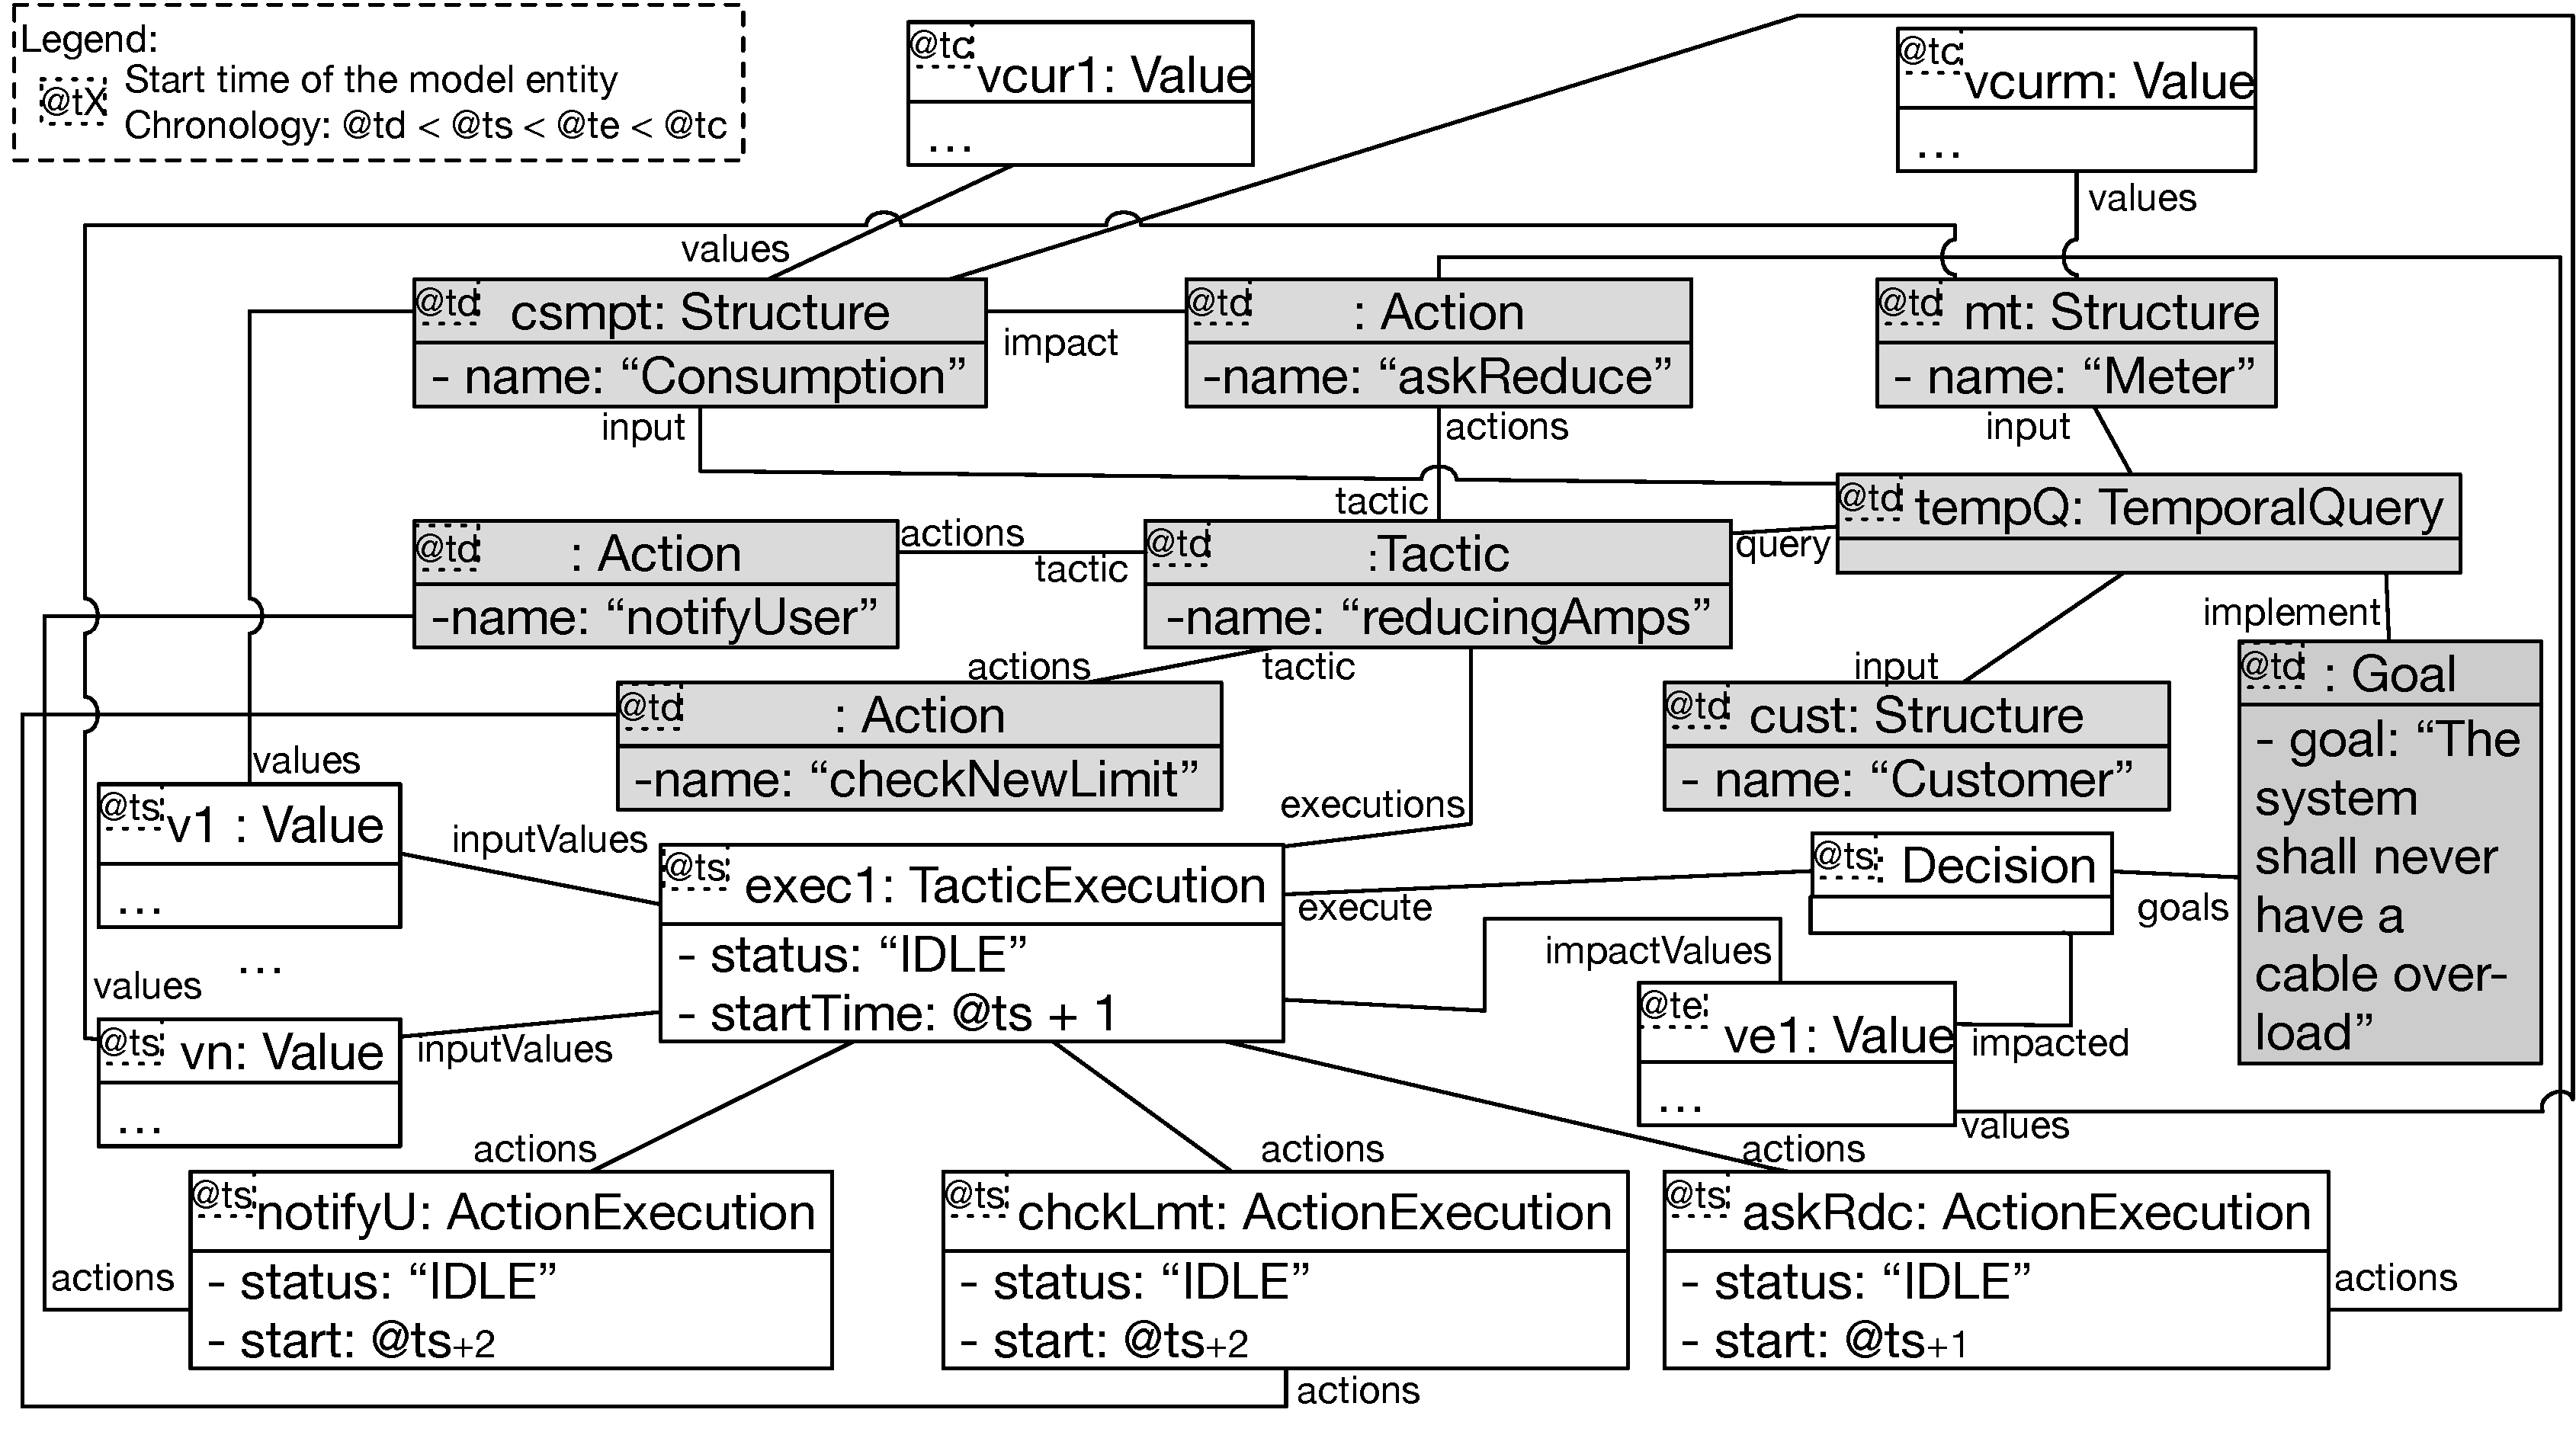
\includegraphics[width=\linewidth]{img/chapt-tkm/validation/action-om}
	\caption{Excerpt of the knowledge object model related to our smart grid example}
	\label{fig:tkm:valid:diag}
\end{figure}

\paragraph{Interactive diagnosis query}
After receiving incident reports concerning regular power cuts, and based on the aforementioned knowledge model, Morgan would be able to query the system's states and investigate why such incidents have occurred.
As described in Section~\ref{sec:tkm:intro:uc}, she/he will interactively diagnose the system by interrogating the context, the decisions made, and their circumstances.

The first function, depicted in Listing~\ref{code:actions-to-goals}, allows  to navigate from the currently measured values (\textit{vcur1}) to the decision(s) made. The for-loop and the if-condition are responsible for resolving the measured data for the past two days. 
Past elements are accessed using the \textit{resolve} function that implements the $Z^T$ relation (\cf Section~\ref{sec:tkm:k-formalism:formalism}).
After extracting the decisions leading to power cuts, Morgan carries on with the diagnosis by accessing the circumstances of this decision. The code to perform this task is depicted in Listing~\ref{code:actions-to-goals}, the second function (getCircumstances).
Note that the relationship \textit{Decision.input} is the aggregation of \textit{Decision.excecute.inputValues}.

\begin{lstlisting}[style=customc,caption=Get the goals used by the adaptation process from executed actions, label=code:actions-to-goals,basicstyle=\scriptsize]
// extracting the decisions
Decision[] impactedBy(Value v) {
  Decision[] respD
  for( Time t: v.modificationTimes() ):
    if (t >= v.startTime() - 2 day)
      Value resV = resolve(v,t)
    respD.addAll(from(resV).navigate(Value.impacted))
  return respD
}
// extracting the circumstances of the made decisions
Tuple<Value[], Goal[]> getCircumstance(Decision d) {
  Value[] resValues = from(d).navigate(Decision.input)
  Goal[] resGoals = from(d).navigate(Decision.goals)      
  return Tuple<>(resValues, resGoals)
} 
\end{lstlisting}

\subsection{Reasoning over unfinished actions and their expected effects}
By associating the action model to the knowledge model, we aim at enhancing adaptation processes with new abilities to reason.
In this section, we present an example of a reasoning algorithm which considers the impacts of running actions.
This example is based on our use case (\cf \Cref{chapt:example}).

Let's imagine that the adaptation process detects overloaded cables in the smart grid.
To fix this situation, it takes several countermeasures, among which there are fuse state modifications.
As detailed in Section~\ref{sec:tkm:intro:motiv}, this action is considered as \gls{longTermAct}.
Later, another incident is detected, for example, a substation is being overloaded.
Before taking any actions, the adaptation process can, thanks to our solution, verify if the running actions will be sufficient to solve this new incident.
If not, it can either take additional actions or replan the running one.
The algorithm to reschedule current actions or to compute additional actions is out of the scope of this thesis.
Here, we present the code to extract the required information from our model.

Checking if the running actions will be sufficient to solve all current issues can also be thought as: will the issue remain with the new context, \ie after each action have been executed.
In our case, it is like verifying if the second overload will still remain with the new topology, which is coming.
The adaptation process, therefore, needs to extract the context in the future.
To do so, the adaptation process should know the latest timepoint at which the impact will be measured.
Listing~\ref{code:tkm:valid:latest-impact} shows the code to get this timepoint.
Running, idle and finished actions are accessed thanks to the first two nested loops with the if-condition.
We consider that failed and canceled actions have no effects.
As finished actions may still have effects, we also consider them.
Then we navigate through all impacted values to get their start time, \ie the beginning of their validity period ($V^T$ relation, \cf Section~\ref{sec:tkm:k-formalism:formalism}).
Doing so, we are sure to get the latest timepoint at which an impact will be measurable.

\begin{lstlisting}[style=customc, caption=Get latest timepoint at which the impact will be measured, label=code:tkm:valid:latest-impact,basicstyle=\scriptsize]
Time latestImpact(Knowledge k) {
  Time latestTime = CURRENT_TIME
  
  for(Decision d: from(k).navigate(decisions))
    for(TacticExecution te: from(d).navigate(execute))
      if(te.status == "RUNNING" || te.status == "IDLE" || te.status == "SUCCEED")
        for(Value v: from(te).navigate(impactedValues))
          if(v.startTime() > latestTime)
            latestTime = v.startTime()
            
  return latestTime
}	
\end{lstlisting}

Using this timepoint, then the adaptation process can then compute how the grid should be after the actions have been executed.
If the system has no prediction mechanism, then the adaptation process can verify how the power will be balanced over the new topology.
Otherwise, it can use this prediction feature to compute the expected loads with the coming topology.
Using this information, it can verify if all current incidents will be solved by the ongoing actions or not.
If not, it may take additional actions or reschedule them.

Listing~\ref{code:tkm:valid:extract-act} depicts the code to extract all running actions.
The nested loops allow accessing all executions made by decision.
Then, we filter only those with the \textquote{RUNNING} status.
The resulting collection should then be given to the scheduling algorithm, which will decide if rescheduling is possible and how. 

\begin{lstlisting}[style=customc, caption=Extract ongoing actions and their effects, label=code:tkm:valid:extract-act,basicstyle=\scriptsize]
TacticExecution[] runningActions(Knowledge k) {
  TacticExecution[] resA
  for(Decision d: k.decisions) {
    for(TacticExecution te: d.execute) {
      if(te.status == Status.RUNNING) {
        resA.add(te)
      }
    }
  }
  return resA
}
\end{lstlisting}

Using our model, developers have two solutions to model a rescheduling operation.
Either they modify the actions, which may delete the history of the previous decision, or they mark all running and idle actions as \textquote{CANCELED} and create a new decision, with new actions, which update the circumstances and re-use the same requirements.

\subsection{Performance evaluation}
GreyCat stores temporal graph elements in several key/value maps. Thus, the complexity of accessing a graph element is linear and depends on the size of the graph. 
Note that in our experimentation we evaluate only the execution performance of diagnosis algorithms. For more information on I/O performance in GreyCat, please refer to the original work by Hartmann \etal~\cite{DBLP:conf/seke/0001FJRT17, DBLP:phd/basesearch/Hartmann16}.

\begin{lstlisting}[style=customc,caption=Traversal used during the experimentations,label=code:traversal-used,basicstyle=\scriptsize]
  MATCH (input)-[*4]->(output)
  WHERE input.id IN [randomly generated set]
  RETURN output
  LIMIT O
\end{lstlisting}

We consider a diagnosis algorithm to be a graph navigation from a set of nodes (input) to another set of nodes (output).
Unlike typical graph algorithms, diagnosis algorithms are simple graph traversals and do not involve complex computations at the node level. Hence, we believe that three parameters can impact their performance (memory and/or CPU): the global size of the graph, the size of the input, and the number of traversed elements.
In our evaluation, we altered these parameters and report on the behaviour of the main memory and the execution time. The code of our evaluation is publicly available online\footnote{https://bitbucket.org/ludovicpapers/icac18-eval}.
All experiments reporting on memory consumption were executed 20 times after one warm-up round. Whilst, execution time experiments were run 100 times after 20 warm-up rounds.
The presented results correspond to the mean of all the iterations.
We randomly generate graph with sizes (\textit{N}) ranging from 1\,000 to 2\,000\,000. 
At every execution iteration, we follow these steps: (1) in a graph with size \textit{N}, we randomly select a set of \textit{I} input nodes, (2) then traverse \textit{M} nodes in the graph, (3) and  we collect  the first \textit{O} nodes that are at four hops from the input element. Listing~\ref{code:traversal-used} describes the behaviour of the traversal using Cypher, a well-known graph traversal language.

We executed our experimentation on a MacBook Pro with an Intel Core i7 processor (2.6 GHz, 4 cores, 16GB main memory (RAM), macOS High Sierra version 10.13.2). We used the Oracle JDK version 1.8.0\_65.

\paragraph{How is the performance influenced by the graph size \textit{N}?}
This experimentation aims at showing the impact of the graph size (\textit{N}) on memory and execution time while performing common diagnosis routines.
We fix the size of \textit{I} to 10. To assure that the behaviour of our traversals is the same, we use a seed value to select the starting input elements. We stop the algorithm when we reach 10 elements.
Results are depicted in Figure~\ref{fig:exp1}.

As we can notice, the graph size does not have a significant impact on the execution time of diagnosis algorithms.
For graphs with up to 2,000,000 elements, execution time remains between 2 ms and four 4 ms. We can also notice that the memory consumption insignificantly increases.
Thanks to the implementation of a lazy loading and a garbage collection strategy by GreyCat, the graph size does not influence memory or execution time performance. The increase in memory consumption can be due to the internal indexes or stores that grow with the graph size.

\begin{figure}
	\centering
	\subfloat[Execution time evolution] {
			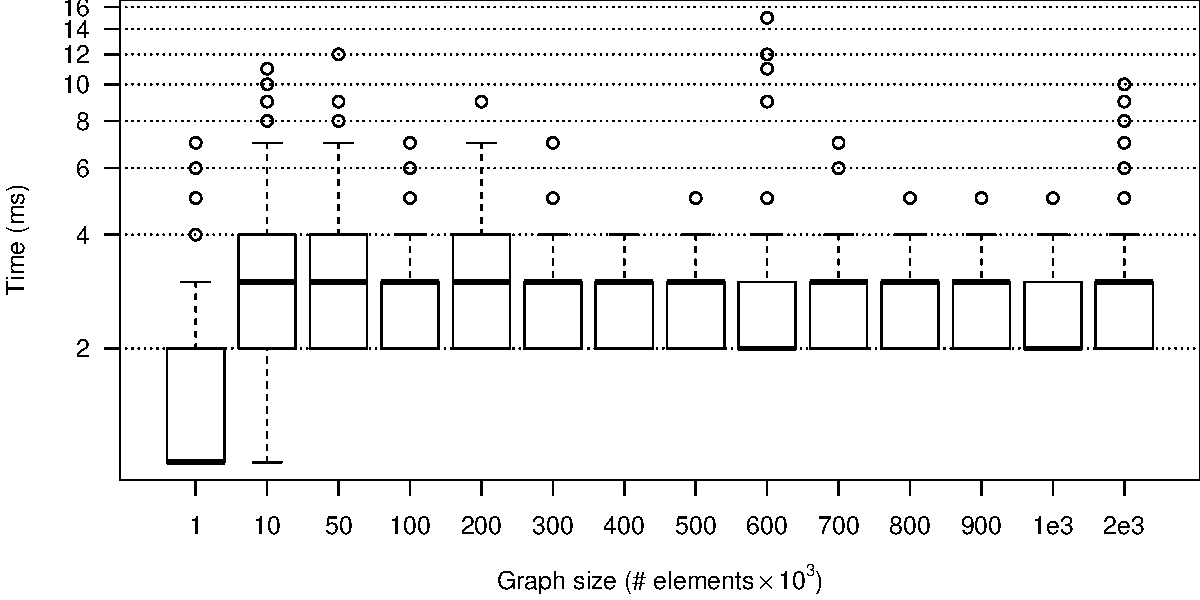
\includegraphics[width=0.85\linewidth]{img/chapt-tkm/validation/exp1-exec-log}
	}
	\hfil
	\subfloat[Memory evolution] {
			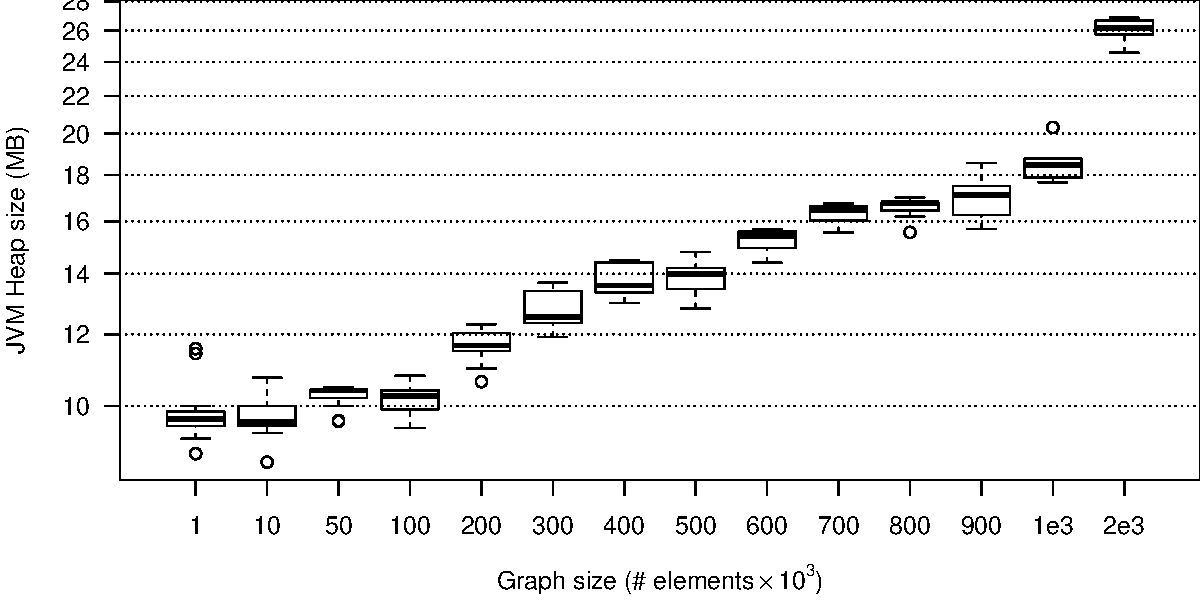
\includegraphics[width=0.85\linewidth]{img/chapt-tkm/validation/exp1-mem-log}
		}	
	\caption{Experimentation results when the knowledge based size increases}
	\label{fig:exp1}
\end{figure}

\paragraph{How is the performance influenced by the input size (I)?}
The second experiment aims to show the impact of the input size (I) on the execution of diagnosis algorithms. We fix the size of \textit{N} to 500\,000 and we variate \textit{I} from 1\,000 nodes to 100\,000, \ie from 0.2\% to 20\% of the graph size. 
The results are depicted in Figure~\ref{fig:exp-res} (straight lines).

Unlike to the previous experiment, we notice that the input size (\textit{I}) impacts the performance, both in terms of memory consumption and execution time. This is because our framework keeps in memory all the traversed elements, namely the input elements.
The increase in memory consumption follows a linear trend with regards to \textit{N}. As it can be noticed, it reaches 2GB for \textit{I}=100\,000. The execution time also shows a similar curve, while the query response time takes around than around 60ms to run for \textit{I}=1\,000, it takes a bit more than 4 seconds to finish for \textit{I}=100\,000. Nonetheless, these results remain very acceptable for diagnosis purposes. 

\paragraph{How is the performance influenced by the number of traversed elements (M)?}%
For the last experiment, we aim to highlight the impact of the number of traversed elements (\textit{M}). For this, we fix \textit{I} and \textit{O} to 1, and randomly generate a graph with sizes ranging from $1\,000$ to $100\,000$. Our algorithm navigates the whole model (\textit{M}=\textit{N}).
We depict the results in Figure~\ref{fig:exp-res} (dashed curve).
As we can notice, the memory consumption increases in a quasi-linear way. The memory footprint to traverse \textit{M} = 100\,000 elements is around 0.9GB. The progress of the execution time curve behaves similarly, in a quasi-linear way. Finally, the execution time of a full traversal over the biggest graph takes less than 2.5 seconds. 

\begin{figure}
	\centering
	\subfloat[Evolution of the execution time]{
		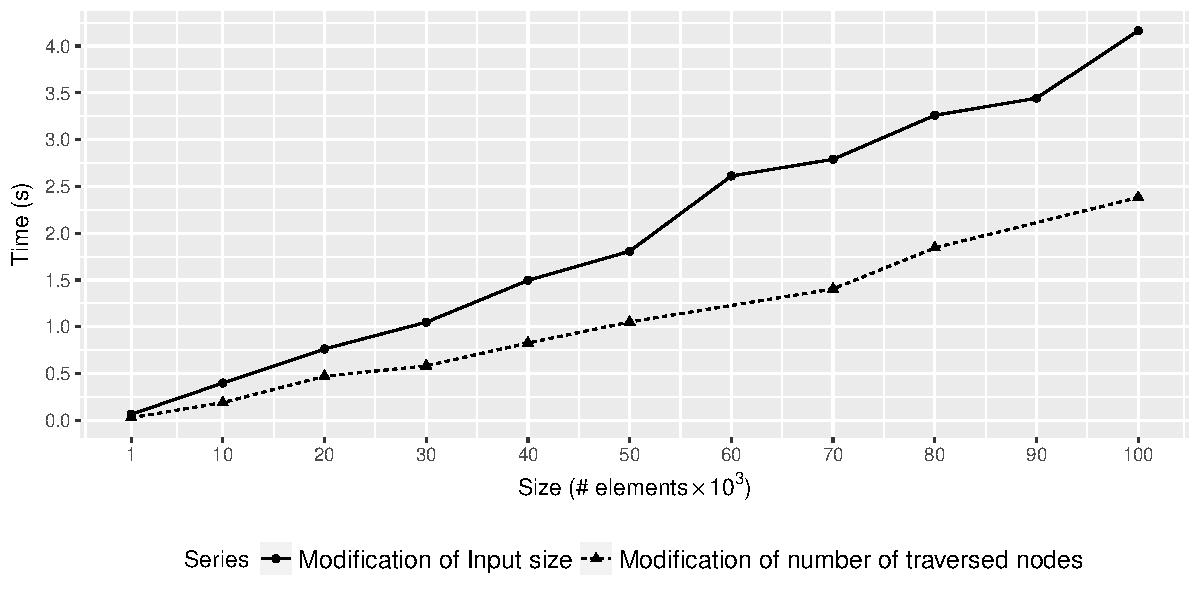
\includegraphics[width=0.9\linewidth]{img/chapt-tkm/validation/exp-exec}
	}
	\hfil
	\centering
	\subfloat[Evolution of the memory consumption]{
		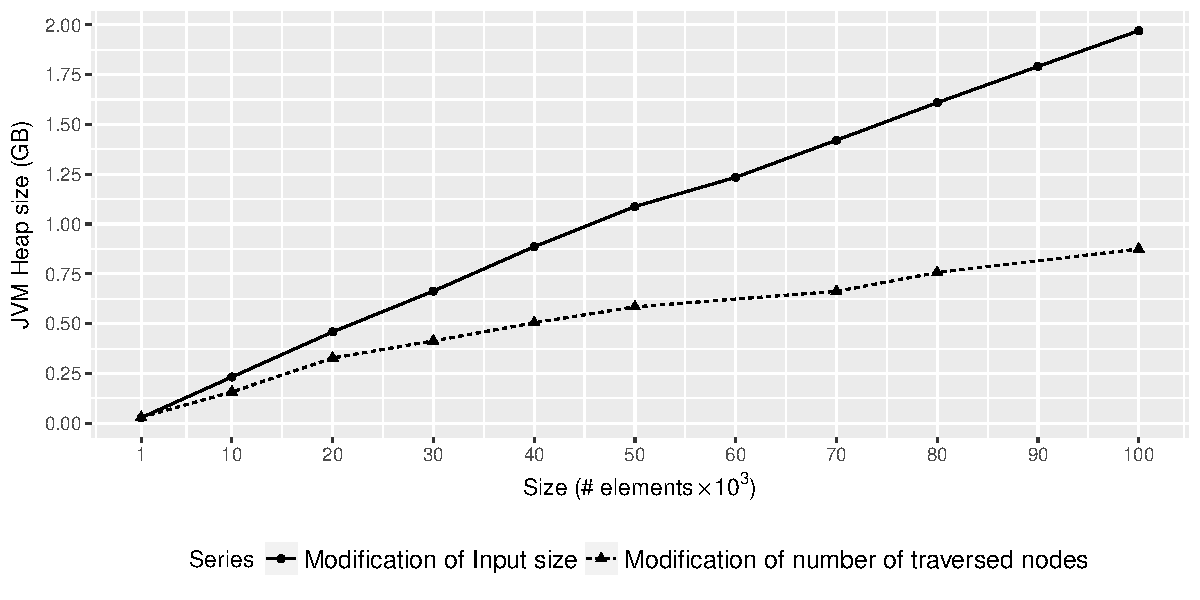
\includegraphics[width=0.9\linewidth]{img/chapt-tkm/validation/exp-mem}
	}
	\caption{Results of experiments when the number of traversed or input elements  increases}
	\label{fig:exp-res}
\end{figure}

\subsection{Discussion}
By linking context, actions, and requirements using decisions, data extraction for explanation or fault localization can be achieved by performing common temporal graph traversal operations.
In the detailed example, we show how a stakeholder could use our approach to define the different elements required by such systems, to structure runtime data, finally, to diagnose the behaviour of adaptation processes. 

Our implementation allows to dynamically load and release nodes during the execution of a graph traversal. Using this feature, only the needed elements are kept in the main memory.  Hence, we can perform interactive diagnosis routines on large graphs with an acceptable memory footprint. 
However, the performance of our solution, in terms of memory and execution time, is restricted by the number of traversed elements and the number of input elements.
Indeed, as shown in our experimentation, both the execution time and the memory consumption grow linearly.

In the Luxembourg smart grid, a district contains approximatively 3 data concentrators and 227 meters\footnote{Previously, our studies uses the data described in \cite{DBLP:conf/smartgridcomm/0001FKTPTR14}, which corresponded to the all Luxembourg at this date. Since 2014, the smart grid has been more and more deployed. Numbers present in this paper now correspond more to one district.}.
Counting the global datacenter, the network is thus composed of 231 elements.
Each meter sends the consumption value every 15 min, being 908 every hours.
Plus, there is from 0 to 273 topology modifications in the network.
In total, the system generates from 908 to 1,181 new values every hour.
If we consider that we have one model element per smart grid entity and one model element per new value, 100,000 model elements correspond thus from $((100,000 - 231) * 1H ) / 1,181 = 84,5H$ ($\sim$ 3,5 days) to $((100,000 - 231) * 1H ) / 908 = 109,9H$ ($\sim$ 4,6 days) of data.
In other word, our approach can efficiently interrogate up to $\sim$5 days history data in 2.4s of one district.

